\section{Introduction}
%
GLIMMER\footnote{{\it GLIMMER} was originally an acronym, reflecting the project's origin within GENIE. The meaning of the acronym is no longer important, however.} is a set of libraries, utilities and example climate drivers used to simulate ice sheet evolution. At its core, it implements the standard, shallow-ice representation of ice sheet dynamics. This approach to ice sheet modelling is well-established, as are the numerical methods used. What is innovative about GLIMMER is its design, which is motivated by the desire to create an ice modelling system which is easy to interface to a wide variety of climate models, without the user having to have a detailed knowledge of its inner workings. This is achieved by several means, including the provision of a well-defined code interface to the model\footnote{The {\it API}, in computer-speak.}, as well as the adoption of a very modular design. The model is coded almost entirely in standards-complient Fortran 95, and extensive use is made of the advances features of that language.
%
\subsection{Overview}
%
GLIMMER consists of several components:
%
\begin{itemize}
\item {\bf GLIDE:} {\bf G}eneral {\bf L}and {\bf I}ce {\bf D}ynamic {\bf E}lements: the core of the model.  This component is the actual ice sheet model. GLIDE is responsible for calculating ice velocities, internal ice temperature distribution, isostatic adjustment and meltwater production. GLIDE needs some representation of the climate to run, provided by a {\it driver} program. The user may write their own driver code, or may use one of the four supplied drivers (see section \ref{subsec:climdrive} below).
\item {\bf SIMPLE:} Simple climate drivers that implement the experiments of the first phase of the EISMINT project, with idealised geometry.
\item {\bf GLINT:} {\bf GL}IMMER {\bf Int}erface. Originally developed for the GENIE\footnote{Grid-ENabled Integrated Earth-system model} Earth Systems Model, GLINT allows the core ice model to be coupled to a variety of global climate models, or indeed any source of time-varying climate data on a lat-long grid. An example driver is provided to illustrate the use of GLINT, which uses temperature and precipitation data to drive a positive degree day (PDD) mass-balance model.
\item {\bf EIS:} {\bf E}dinburgh {\bf I}ce {\bf S}heet climate driver based on a parameterisation of the equilibrium line altitude, sea-level surface temperatures and eustatic sea-level change.
\item {\bf EISMINT3:} An implementation of a later part of the EISMINT project, concerning the modelling of the Greenland ice sheet.
\item {\bf GLUM:} {\bf G}Limmer {\bf U}seful {\bf M}odules, various utility procedures used by the other components.
\item Visualisation programs using GMT\footnote{Generic Mapping Tools}.
\end{itemize}
%
\begin{figure}[htbp]
  \centering
  \includegraphics[width=0.6\textwidth]{\dir/figs/glimmer.eps}
  \caption{Relationship between the various GLIMMER components.}
  \label{ug.fig.glimmer}
\end{figure}
The relationship between the GLIMMER components is illustrated in Figure \ref{ug.fig.glimmer}.
%
\subsection{Climate Drivers}
\label{subsec:climdrive}
The core ice sheet model, GLIDE, is connected to the climate via the surface mass balance and temperature fields and (optionally) a scalar value for eustatic sea level. These drivers can be derived from simple assumptions, e.g. uniform mass balance or EISMINT tests, or from climate model output, e.g. GENIE or a regional climate model. These components, and how they relate to each other, are outlined in Figure \ref{ug.glide}.
%
\begin{figure}[htbp]
 \begin{center}
   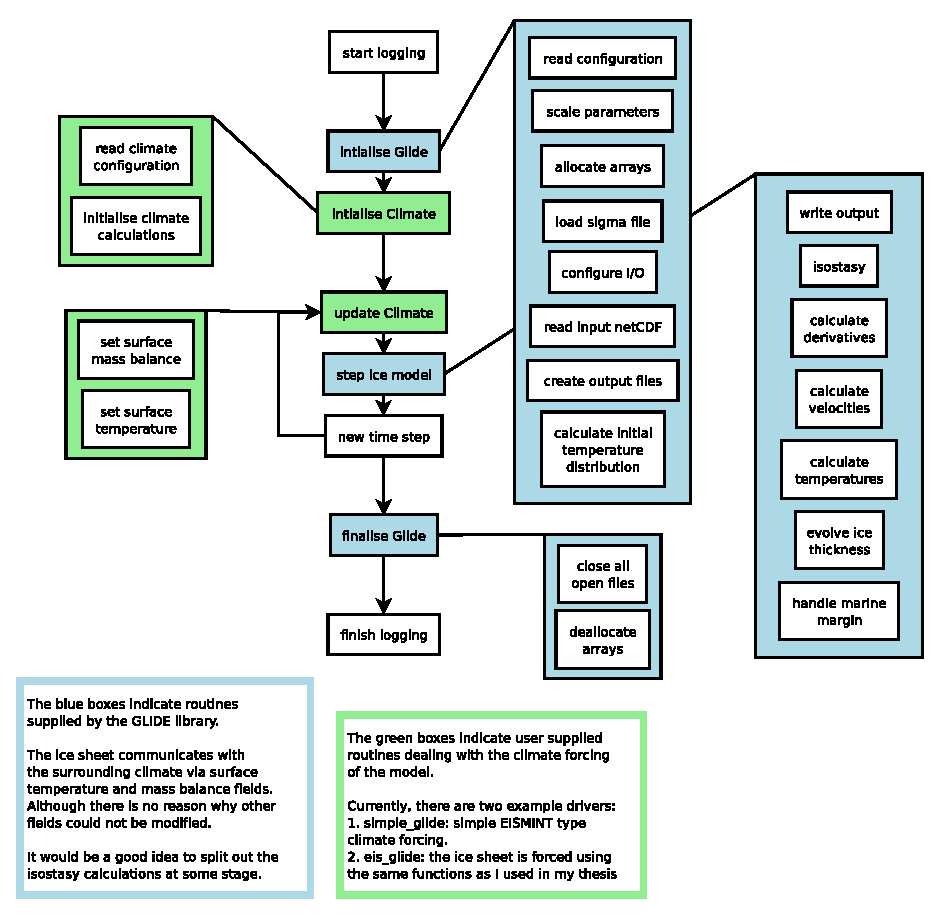
\includegraphics[width=0.9\textwidth]{\dir/figs/glide.eps}
 \end{center}
 \caption{Outline of the GLIDE and Climate components.}
\label{ug.glide}
\end{figure}
%
\subsection{Configuration, I/O and Visualisation}
In general terms, each component is configured using a configuration file similar to Windows \texttt{.ini} files. At run-time, model configuration is printed to a log file. 

2D and 3D data is read/written to/from netCDF files using the CF (Climate-Forecast) metadata convention\footnote{\texttt{http://www.cgd.ucar.edu/cms/eaton/cf-metadata/}}. NetCDF is a scientific data format for storing multidimensional data in a platform- and language-independent binary format. The CF conventions specify the metadata used to describe the file contents.

Many programs can process and visualise netCDF data, e.g. OpenDX, Matlab, IDL, etc. Additionally, the GLIMMER code bundle contains GMT scripts written in Python to visualise the output.
